\documentclass{ies2018}
\usepackage{amsmath}
\usepackage{graphicx}
\usepackage{algorithm}
\usepackage{algorithmic}
\usepackage{subfigure}
%% Put title here
\title{Distributed Bat Algorithms adjusting Direction and Distance between Solutions for Multimodal Optimization}

%% List authors here
\author{Takuya Iwase $^{\dagger}$ \and Ryo Takano $^{\dagger}$ \and Fumito Uwano $^{\dagger}$ \and Hiroyuki Sato $^{\dagger}$ \and Keiki Takadama $^{\dagger}$}
%% Authors' affiliations
\affiliation{%
    ${}^\dagger$ The University of Electro-Communications, Tokyo, Japan\\
    % ${}^\ddagger$ University/Company, City, Country
}
%% Contact email address
\email{tanu_iwa@cas.lab.uec.ac.jp}

%% Put abstract here
\abstract{%
    This paper proposes new algorithms for finding multiple optima in multimodal optimization, which k-nearest neighbor bat algorithm (k-NNBA) and novelty search-based bat algorithm (NSBA). Conventional algorithms of swarm intelligence tend to straightforward converge a global optimum or a local optimum of high-fitness value. However finding local optima is important because local optima might become better solutions or a new global optimum due to make search domain changed in real world problems. In this paper, bat algorithm (BA) which is available to change exploration and exploitation performance automatically using the characteristic of echolocation, is extended with k-nearest neighbor and novelty search for keeping the distance between each solution, and we validate the performance used multimodal functions. 
}%
%% with relevant keywords
\keywords{Multimodal Optimization, Swarm Intelligence, Bat Algorithm}


\begin{document}

\maketitle

\section{Introduction}

In the past couple of decades, metaheuristic algorithms became major method for optimization problem. Generally, these algorithms are based on biological evolution in nature-inspired system. These algorithms are adaptable for metaheuristic optimization using non-linear objective functions. For example, Particle Swarm Optimization (PSO) is modeled fish swarm if one fish find a single global optimum, the other fishes converge to the fish \cite{PSO01}. Meanwhile, another algorithm called Firefly Algorithm (FA), which is particularly well for exploitation with flashing light of fireflies \cite{FA01}. In two fireflies, a brighter firefly attracted the other one. Bat algorithm (BA) also one of metaheuristic algorithms is available to switch exploration and exploitation automatically with characteristic of echolocation \cite{BA01}. All bats move to a bat which found food or prey, with loudness and pulse rate to sense the distance each other. Simultaneously, some of them fly randomly for searching the other prey globally. After finding a prey, they will drop loudness down and raise pulse rate up automatically, for adjusting to search spatial domain. However considering for dealing with real-world problems which has many multiple optima in search domain, these algorithms are not adaptable because they tend to converge a single global optimum without keeping local optima.
% Although these algorithms are widely used for optimization problem, the performance of search considerably depends on the scale and contour of multimodal functions. To adapt any optimization problem, we have to consider the balance of performance which unites global search and local search.
 
 % The bat behavior is determined echolocation which is sound wave for finding food in the dark. Ideally 
  However, the performance of global search is still higher than local search, bat algorithm is easily fallen global minimum or high-fitness value on multimodal problems. For this reason, we propose distributed BA (k-NNBA and NSBA) for migrating solutions away and keeping distance each other. Besides for the performance measurement, we set different changes: (a) for guiding local search using personal best solution or previous position of solution instead of global best solution; (b) existence or nonexistence of a new solution generated by flying randomly. 
 % The reasons for multimodal optimization are to find the global optimum definitely, and the other local optima of high-fitness solutions. 
 % There are several approaches for this reasons, which based on Genetic Programming(GP) \cite{GPharada}, PSO \cite{PSO4mo}\cite{PSO4mo2} and Differential Evolutionary(DE) \cite{DE4mo}\cite{DE4mo2}. However, for practical optimization problems, it is desirable to use multimodal functions to reach the peak of both global optima and local minima located, with small population size.  \\
This paper is composed of 7 sections. After introduction, we demonstrate mechanism of conventional BA and proposed BA in 2nd and 3rd section. In 4th section, we describe about the experiment using the multimodal functions and parameters. Followed by results in 5th section, we discuss about the results in 6th section, conclusion is 7th section finally.

\section{Bat Algorithm}
BA based on microbat behavior uses frequency and loudness for adaptive global search on a multimodal function.
 % In this algorithm, loudness ${A^0}$ is used as a parameter to adjust frequency. 
 When microbat moves toward target, loudness ${A^0}$ is gradually decreased in proportion to travel distance of microbat decreases. Behavior of microbat is consists of following three rules: 

\begin{itemize}
\item Each bat measures the distance between its own location and target using frequency ${f_i}$.
\item At the location ${x_i}$, each bat with velocity ${v_i}$ moves toward target randomly.
\item Loudness ${A^0}$ varies to sense how far approaching toward the target.  
\end{itemize}

Each bat with velocity ${v_i}$, location ${x_i}$, and frequency ${f_i}$ is defined as follows:
\begin{equation}
f_{i} =f_{min}+(f_{max}-f_{min}) \beta
\label{eq:freq} 
\end{equation}
% \begin{equation}
% d_i^{t-1}=x_*-x_i^{t-1}
% \label{eq:d}
% \end{equation}
\begin{equation}
v_i^t=v_i^{t-1}+(x_*-x_i^{t-1})* f_i
\label{eq:vel}
\end{equation}
\begin{equation}
x_i^t=x_i^{t-1}+v_i^t
\label{eq:xi}
\end{equation}

Velocity ${v_i}$ controlled by tuning frequency ${f_i}$ from [${f_{max}}$ ${f_{min}}$] as ${f_{max}}=1$ and ${f_{min}}=0$. $\beta $ is uniform random distribution from 0 to 1. In global search step, each bat moves to location ${x_i}$ with velocity ${v_i}$ toward global best solution
% , as shown in Fig. \ref{fig:bbat}
. Secondly in local search step, a new candidate solution ${x_{new}}$ is generated around a global best solution
% , as shown 2nd phase of Fig. \ref{fig:bbat}
. The equation as below

\begin{equation}
x_{new}=x_{*}+ \epsilon A^t \ ,
\label{eq:loc}
\end{equation}

where ${\epsilon}$ is uniform random distribution between ${[0,  \ 1]}$. ${A^t}$ is the average loudness of all bats. Initialized all bats start searching target using loudness ${A_i}$ and the reflect wave as pulse emission rate ${r_i}$. Loudness and pulse rate are updated as follows:

\begin{equation}
A_i^{t+1}=\alpha A_i^t
\label{eq:A}
\end{equation}
\begin{equation}
r_i^{t+1}=r_i^0[1-exp(-\gamma t)]
\label{eq:r}
\end{equation}

These parameters are also updated when a new candidate solution is updated by equation (\ref{eq:loc}) for each iteration. Loudness gradually decreases as approaching to a target, pulse rate increases in contrast. BA initializes pulse rate as a uniform random distribution ${r_i^0}$ between ${[0, \ 1]}$ or a number closed around zero. ${\alpha}$ and ${\gamma}$ are symbolized damping coefficient. In simulated experiment, these coefficient parameters are set ${\alpha = \gamma = 0.9}$. The pseudo code and the process of BA presented as below.
 % (shown in Fig. \ref{fig:bbat} \& Algorithm \ref{code:ba}).
% \begin{figure}[h]
% \begin{center}
% 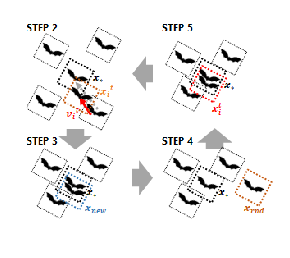
\includegraphics[width=1.0\linewidth]{eps/bbat_motion.eps}
% \end{center}
% \caption{Bat Motion of BA}
% \label{fig:bbat}
% \end{figure}

\begin{itemize}
\item STEP1: Initialize population of bats (line 1 to 3)\\
Initialize location ${x_i}(i=1, 2, ..., n)$ with velocity ${v_i}(i=1, 2, ..., n)$ randomly. Each bat has loudness ${A_0}$, parse rate ${r_i}$ and frequency ${f_i}$ as initial value.
\item STEP2: Generate new solutions (line 6 to 7)\\
Generate new solutions ${x_i^t}$ based on equation (\ref{eq:xi}).
\item STEP3: In local search phase, Generate a new solution around global best solution ${x_*}$ (line 8 to 12)\\
In case of a random distribution higher than parse rate ${r_i}$, generate a new solution ${x_{new}}$ around ${x_*}$.
\item STEP4: Generate a new solution randomly (line 13)\\
Generate a new solution ${x_{rnd}}$ by random generation of bat.  
\item STEP5: Rank and update solutions (line 14 to 17)\\
In case of ${rand < A_i}$, choose the best from all solutions which are ${x_i, x_{new}}$, and ${x_{rnd}}$, and cross over as personal best solution unless it is higher than the value of former iteration.  
\item STEP6: Loop to STEP2 
\end{itemize}

\begin{algorithm}[H]
\caption{Bat Algorithm}
\label{code:ba}
\begin{algorithmic}[1]
\REQUIRE $Objective\ Function\ f(x)$
\STATE Initialize Population $x_i(i=1,2,..., n)$ and $v_i$\\
\STATE Define frequency $f_i$ at location $x_i$ \\
\STATE Initialize pulse rates $r_i$, and loudness $A_i$
\WHILE{($t <$ Max number of iterations)}
\FOR{i=1 to n}
\STATE Generate new solutions $x_i$ by tuning frequency $f_i$
\STATE Update location $x_i$ and velocity $v_i$  [eqs.(\ref{eq:freq}) to (\ref{eq:xi})]
\IF{($rand>r_i$)}
\STATE Generate a new solution $x_{new}$ around global best solution $x_i$ [eq.(\ref{eq:loc})] 
% \ELSE
% \STATE Continue
\ENDIF
\STATE Generate a new solution $x_{rnd}$ randomly
\IF{($rand<A_i \& {f(x_i), f(x_{new}), f(x_{rnd})}<f(x_*)$)}
\STATE Accept the new solution, and update pulse rate $r_i$ \\ \& loudness $A_i$ [eqs. (\ref{eq:A})(\ref{eq:r})]  
\ENDIF
\STATE Evaluate all bats and select a best solution $x_*$ in the current solutions
\ENDFOR
\ENDWHILE
\end{algorithmic}
\end{algorithm}

\section{Distributed Bat Algorithm}
For reaching local and global minima,it is necessary to make bats spread widely. In k-nearest neighbor bat algorithm (k-NNBA), we focus on difference between the number of population. In Novelty Search-based bat algorithm (NSBA), we consider as written the difference above, and distance of each bat.
\subsection{k-Nearest Neighbor Bat Algorithm}
k-nearest neighbor (k-NN) method is used for classification for data with discrete label basically. The mechanism of k-nearest neighbor is to find a new object (a new point) with closest distance between the other objects around it, and predict discrete label from these factors. Here, we use a new object as a new solution with the distance for keeping each bat away. The distance equation is written as below.

\begin{equation}
d_i^{t-1}=\frac{1}{K}\sum_{j=1}^K {(x_{i*}-x_j^{t-1})}
\label{eq:kd*}
\end{equation}
\begin{equation}
d_i^{t-1}=\frac{1}{K}\sum_{j=1}^K {(x_i^{t-1}-x_j^{t-1})}
\label{eq:kdi}
\end{equation}

K describes the number of nearest neighbor. In equation (\ref{eq:nd*}), ${x_{i*}}$ means personal best solution. k-NN is very simple method and is easy to implement, but depending on number of neighbors, we have to choose proper k. Pseudo code is described in Algorithm 2.


\subsection{Novelty Search-based Bat Algorithm}
\subsubsection{Novelty Search}
Novelty search is used as evolutionary search approach to expand dense solutions into sparse area and to measure the distance between current solutions to reward or delete it. The sparseness of solutions is calculated as below,
\begin{equation}
\rho(x)=\frac{1}{k}\sum_{i=0}^k dist(x,\mu_i),
\label{eq:nov}
\end{equation}
where the sparseness ${\rho(x)}$ at a point ${x}$ shows the scatter of solutions. The dist in k-nearest neighbors is the average distance between the point ${x}$ and ${\mu_i}$, which is the ${i}$th nearest neighbor of ${x}$. This is an example in case of k neighbor = 3 (shown in Fig. \ref{fig:n_dist}). It describes that a solution is migrated away from three neighbors. 

\begin{figure}[h]
\begin{center}
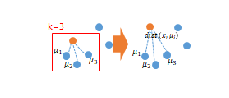
\includegraphics[width=1.0\linewidth]{eps/n_dist.eps}
\end{center}
\caption{distributed a solution to sparse area}
\label{fig:n_dist}
\end{figure}

\subsubsection{Novelty Search-based Bat Algorithm}
In order to adapt multimodal optimization not only single objective optimization, Novelty Search-based Bat Algorithm (NSBA) enables all population to reach local minima. This paper proposes a method of keeping over a certain distance between each location of bat, and letting population remain around local minima. Using this behavior, all population are updated by the equation as bellow, 
\begin{equation}
d_i^{t-1} = \frac {1}{K} \sum _{j=1}^K \frac {(x_{i*}-x_j^{t-1})}{|x_{i*}-x_j^{t-1}|^2}
\label{eq:nd*}
\end{equation}
\begin{equation}
d_i^{t-1}=\frac{1}{K}\sum_{j=1}^K \frac{(x_i^{t-1}-x_j^{t-1})}{|x_i^{t-1}-x_j^{t-1}|^2}
\label{eq:ndi}
\end{equation}

where ${K}$ is population size of nearest neighbor, and ${x_{i*}}$ indicates personal best solution. ${x_i^{t-1}}$ is previous position of solution. In addition, bats with velocity ${v_i^t}$ and location ${x_i^t}$ are updated same as (\ref{eq:vel}) and (\ref{eq:xi}) of conventional method. Used distance function in Novelty search describes scalar equation. However in this proposes, we alter scalar to vector equation for determining search direction. 

 \subsubsection{Distance of each bat} 
 Above-mentioned the vector equation \ref{eq:kd*} and \ref{eq:kdi}, as distance of each bat is closer, they hardly move to sparse area. Conversely, as they located far away each other, they move greatly up to a boundary of search area. To control this movement, we introduce the denominator as equation (\ref{eq:nd*})(\ref{eq:ndi}). Here is the Algorithm flow on global minimum optimization. The NSBA pseudo code is described in Algorithm 2.

\begin{itemize}
\item STEP1: Initialize population of bats (line 1 to 3)\\
Initialize location ${x_i}(i=1, 2, ..., n)$ with velocity ${v_i}(i=1, 2, ..., n)$ randomly. Each bat has loudness ${A_0}$, parse rate ${r_i}$ and frequency ${f_i}$ as initial value.
\item STEP2: Generate new solutions (line 6 to 7)\\
Generate new solutions ${x_i^t}$ based on equation (\ref{eq:vel})(\ref{eq:xi}) with (\ref{eq:ndi}) or (\ref{eq:nd*}).
\item STEP3: In local search phase, Generate a new solution around solutions ${x_i}$ (line 8 to 12)\\
In case of a random distribution higher than parse rate ${r_i}$, generate a new solution ${x_{local}}$ around ${x_i}$.
\item STEP4: Generate a new solution randomly (line 13)\\
Generate a new solution ${x_{rnd}}$ by random walk of bat.  
\item STEP5: Rank and update solutions (line 14 to 18)\\
If ${rand < A_i}$, choose the best from all solutions which are ${x_i, x_{local}}$, and ${x_{rnd}}$. After that, cross over as personal best solution unless it is higher fitness value than previous iteration.  
\item STEP6: Loop to STEP2
\end{itemize}

\begin{figure}[h]
\begin{center}
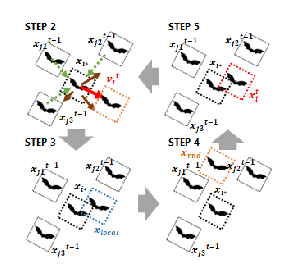
\includegraphics[width=1.0\linewidth]{eps/sbat_motion.eps}
\end{center}
\caption{Bat motion of NSBA}
\label{fig:sbat}
\end{figure}

\begin{algorithm}[H]
\caption{Distributed Bat Algorithm}
\label{code:sba}
\begin{algorithmic}[1]
\REQUIRE $Objective\ Function\ f(x)$
\STATE Initialize Population $x_i(i=1,2,..., n)$ and $v_i$\\
\STATE Define frequency $f_i$ at location $x_i$ \\
\STATE Initialize pulse rates $r_i$, and loudness $A_i$
\WHILE{($t <$ Max number of iterations)}
\FOR{i=1 to n}
\STATE Generate new solutions $x_i$ by tuning frequency $f_i$
\STATE Update location $x_i$, velocity $v_i$  [eqs.(\ref{eq:freq})(\ref{eq:vel})(\ref{eq:xi})] \\ and k-NNBA for [eq.(\ref{eq:kd*})(\ref{eq:kdi})] NSBA for [eq.(\ref{eq:nd*})(\ref{eq:ndi})] 
\IF{($rand>r_i$)}
\STATE Generate a new solution ${x_{local}}$ around the solution $x_{i}$ [eq.(\ref{eq:loc})] 
\ELSE
\STATE Continue
\ENDIF
\STATE Generate a new solution $x_{rnd}$ randomly (or without ${x_{rnd}}$)
\IF{($rand<A_i \& f(x_i)<f(x_i)$)}
\STATE Accept the new solution, and update pulse rate $r_i$ \\ \& loudness $A_i$ [eqs. (\ref{eq:A})(\ref{eq:r})]  
\ENDIF
\ENDFOR
\STATE Evaluate the all bats and select a best solution $x_i*$ in the current solutions
\ENDWHILE
\end{algorithmic}
\end{algorithm}

\subsection{Comparion with k-NNBA and NSBA}
we compare 8 methods in total. There are comparison of these methods on below Table \ref{tb:compare}.  
\begin{table}[h]
\begin{center}
\caption{Comparion with k-NNBA \& NSBA}
\label{tb:compare}
\begin{tabular}{c|c|c|c|c}
\hline 
\multicolumn{1}{c|}{${x_{rnd}}$} & \multicolumn{2}{c|}{$\circ$} & \multicolumn{2}{c}{$\times$}   \\
\hline
 x & ${x_{i*}}$ & ${x_i^{t-1}}$ & ${x_{i*}}$ & ${x_i^{t-1}}$ \\
\hline 
k-NNBA & I & II & III & IV\\
NSBA & V & VI & VII & VIII\\
\hline
\end{tabular}
\end{center}
\end{table}

\section{Multimodal Function}
 In the contour of function, there are the coordinate that horizontal axis is x1 and vertical axis is x2, and the colorbar that color density describes the fitness value shown as Fig. \ref{fig:cgf}. As color becomes darker area, fitness value gets lower. For validating NSBA to distribute spread widely, there are some multimodal functions. Focused on depth of fitness value, scale of multimodal domain and number of local minima, we used these functions as following section.  
\subsection{Griewank Function}
As an example to demonstrate the bat motion of this algorithm, we use Griewank function as below (shown in Fig. \ref{fig:3dgf})
\begin{equation}
f(x)= \sum_{i=1}^d \frac{x_{i}}{4000} - \prod_{i=1}^d \cos(\frac{x_i}{\sqrt{i}}) + 1,
\end{equation}
where global optimum is ${f(x_*)}=0$, at $x_* = {[0 \ \ 0]}$. There are 17 local minima at ${\pm x \approx}$ ${ [6.2800 \ \ 8.8769],}$ ${[3.1400 \ \ 4.4385],}$ \\ ${[0 \ \ 8.8769]}$, ${[6.2800 \ \ 0], [9.4200 \ \ 4.4385]}$ in the range of this function is between ${-10 \leq x_i \leq 10}$ with i=1,2,...,d. The function ${f(x)}$ has global minimum ${f(x_*)}=0$ and also the other local minima ${f(x_{i*)} \approx 0}$  for ${d=2}$.  

 \subsection{Rastrigin Function}
 This function has 121 local minima in the spatial domain, at ${ \pm x=}$ ${[0,...,11 \ \ 0,...,11]}$. And global minimum is ${f(x_*)=0}$ at ${x=[0 \ \ 0]}$. The function equation is
 \begin{equation}
f(x)= 10d+\sum_{i=1}^d [x_i^2-10 \cos(2\pi x_i)]
\end{equation}
3D model and contour of this function are showed in Fig. \ref{fig:3drf} \& \ref{fig:crf}. 

\begin{figure}[h]
\centering
\subfigure[Fitness landscape]{
\includegraphics[width=0.8\linewidth]{eps/3d_griewank.eps}
\label{fig:3dgf}}
\subfigure[Contour plot]{
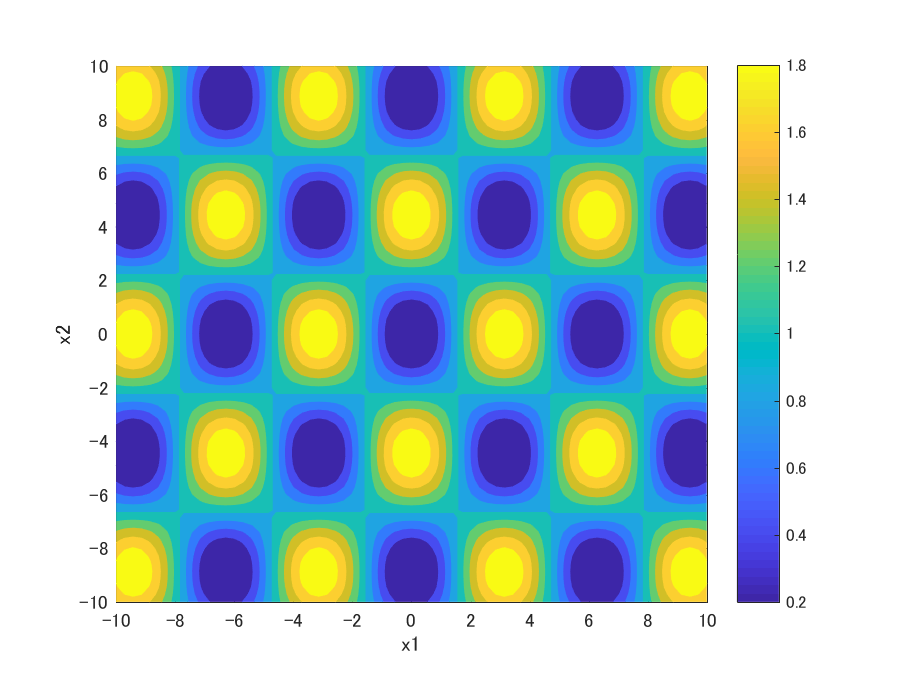
\includegraphics[width=0.8\linewidth]{eps/cont_griewank.eps}
\label{fig:cgf}}

\caption{Griewank Function}
\label{fig:3d}
\end{figure}

\begin{figure}[h]
\centering
\subfigure[Fitness landscape]{
\includegraphics[width=0.8\linewidth]{eps/3d_rastrigin.eps}
\label{fig:3drf}}
\subfigure[Contour plot]{
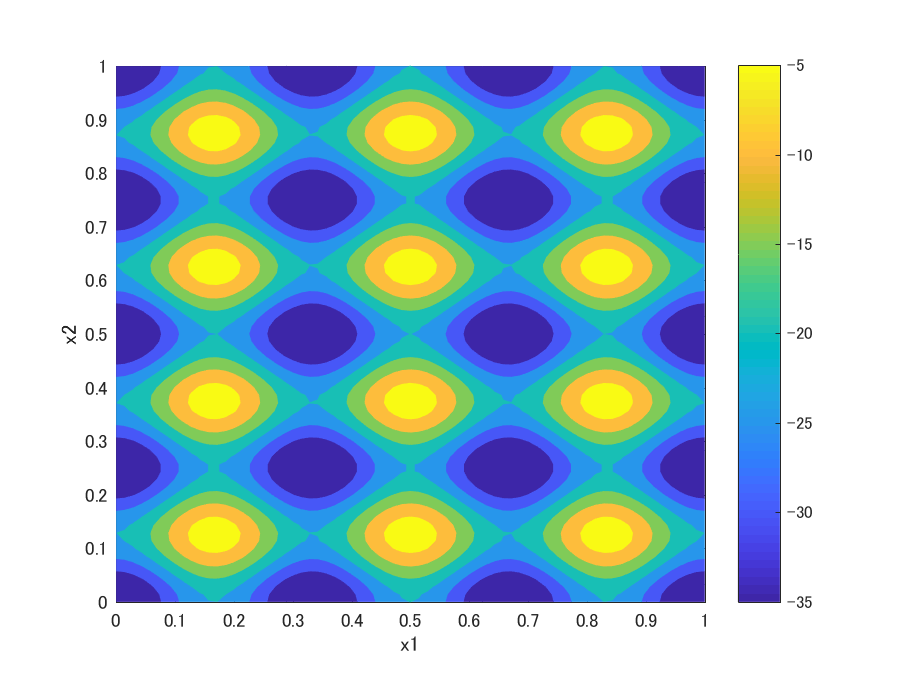
\includegraphics[width=0.8\linewidth]{eps/cont_rastrigin.eps}
\label{fig:crf}}

\caption{Rastrigin Function}
\label{fig:cf}
\end{figure}

\section{Experiment}
 We compared proposed NSBA with the other algorithms, which NNBA and BA. Each algorithm was run for 10 seeds to validate the performance of NSBA. In this paper, the algorithm is implemented on MATLAB for the benchmark function.

\subsection{Evaluation Criteria}
$dist$ is total amount of the distance between local minima and nearest neighbor population, in case of initializing population randomly each algorithm. In this experiment, we focus on how many found local minima, and $dist$ which total amount of the distance between local minima and the closest solutions, as below. \\
\begin{equation}
dist=\sum_{i=1}^M {min_{j \in N}|s_i-x_j|},
\label{eq:dist}
\end{equation}
 where ${M}$ is maximum number of local minimum, and ${N}$ is population size of bats. ${s_i}$ means the coordinate of local minimum. As ${dist}$ is closed zero, the number of bats located local minima increases. We compare with the performance of these algorithms in term of the population size and the bat behavior by iteration. 

\subsection{Experimental Parameter}
All experiments use same parameters, where population size ${N=20}$, frequency ${f_{max}=1, f_{min}=0}$, loudness ${A^0}=1$, parse rate ${r^0} \in [0 \ \ 1]$ with ${\alpha =\gamma = 0.9}$.

\subsection{Result}
 \subsubsection{Comparison with I and V}
On griewank function, dist of k-NNBA and NSBA are nearly same in any neighbors, but k-NNBA is slightly better performance than NSBA on each function. From rastrigin function, k-NNBA is smaller than NSBA in any neighbors.

\subsubsection{Comparison with II and VI}
On griewank function, NSBA is almost better than k-NNBA in each neighbor except for K=4, dist of k-NNBA is a bit smaller. Overall, ${dist}$ is higher than the other methods on griewank function. In rastrigin function, k-NNBA gradually increased. However, NSBA slowly decreased until K=16.

\subsubsection{Comparison with III and VII}
Method III and VII are better performance than the other mothods in griewank function.
However, k-NNBA became worse as increasing neighbors. By contrast, NSBA was very unchanged in any neighbors. Besides, averages of k-NNBA and NSBA almost unchanged.  

 \subsubsection{Comparison with IV and VIII}
The dist of NSBA is smaller than k-NNBA in K=2 to 20 on both functions, except for K=2 and 4 on rastrigin function. The average of NSBA also smaller than k-NNBA. 
 Comparison to NSBA in Fig. \ref{fig:*bar_func}, dist of k-NNBA is lowest of the other number of neighbors. However, dist of k-NNBA rose up gradually from K=4. By contrast, dist of NSBA remains fairly on griewank function, but the performance gets worse after K=4. Overall, 

\begin{figure}[p]
\centering
\subfigure[Griewank Function]{
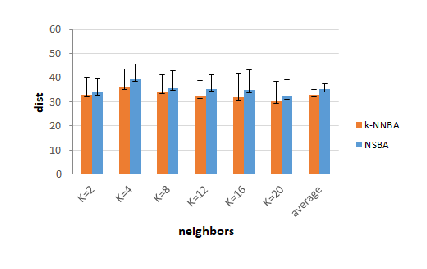
\includegraphics[width=0.4\textwidth]{eps/pbest_grie_r.eps}
\label{fig:r*bar_grie}}

\subfigure[Rastrigin Function]{
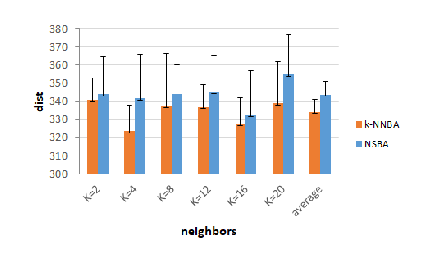
\includegraphics[width=0.4\textwidth]{eps/pbest_rast_r.eps}
\label{fig:r*bar_rast}}
\caption{Comparison with method I \& V}
\label{fig:r*bar_func}
\end{figure}

\begin{figure}[p]
\centering
\subfigure[Griewank Function]{
\includegraphics[width=0.4\textwidth]{eps/t-1_grie_r.eps}
\label{fig:rtbar_grie}}

\subfigure[Rastrigin Function]{
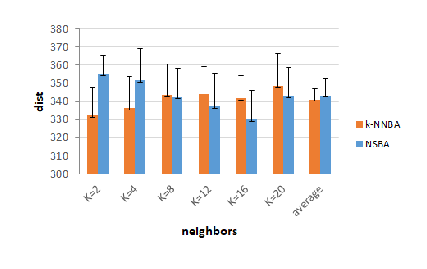
\includegraphics[width=0.4\textwidth]{eps/t-1_rast_r.eps}
\label{fig:rtbar_rast}}
\caption{Comparison with method II \& VI}
\label{fig:rtbar_func}
\end{figure}

\begin{figure}[p]
\centering
\subfigure[Griewank Function]{
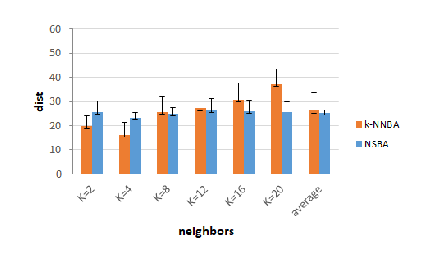
\includegraphics[width=0.4\textwidth]{eps/pbest_grie.eps}
\label{fig:*bar_grie}}

\subfigure[Rastrigin Function]{
\includegraphics[width=0.4\textwidth]{eps/pbest_rast.eps}
\label{fig:r*bar_rast}}
\caption{Comparison with method III \& VII}
\label{fig:*bar_func}
\end{figure}

\begin{figure}[p]
\centering
\subfigure[Griewank Function]{
\includegraphics[width=0.4\textwidth]{eps/t-1_grie.eps}
\label{fig:tbar_grie}}

\subfigure[Rastrigin Function]{
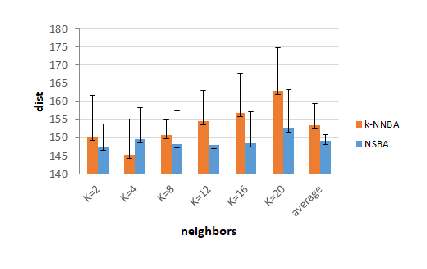
\includegraphics[width=0.4\textwidth]{eps/t-1_rast.eps}
\label{fig:rtbar_rast}}
\caption{Comparison with method IV \& VIII}
\label{fig:tbar_func}
\end{figure}



\begin{figure}[p]
\centering
\subfigure[k-NNBA]{
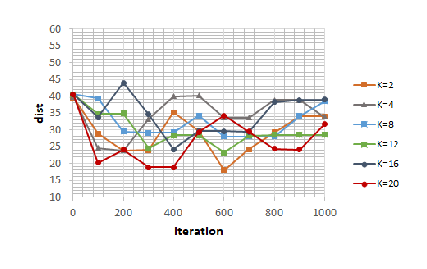
\includegraphics[width=0.4\textwidth]{eps/ip_k_r.eps}
\label{fig:ri*_k}}

\subfigure[NSBA]{
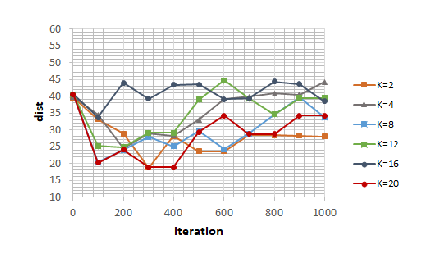
\includegraphics[width=0.4\textwidth]{eps/ip_ns_r.eps}
\label{fig:ri*_ns}}
\caption{Comparison with method I \& V}
\label{fig:ri*_iter}
\end{figure}

\begin{figure}[p]
\centering
\subfigure[k-NNBA]{
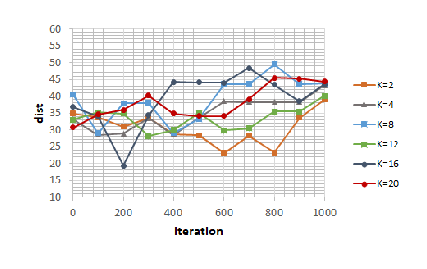
\includegraphics[width=0.4\textwidth]{eps/it-1_k_r.eps}
\label{fig:rit_k}}

\subfigure[NSBA]{
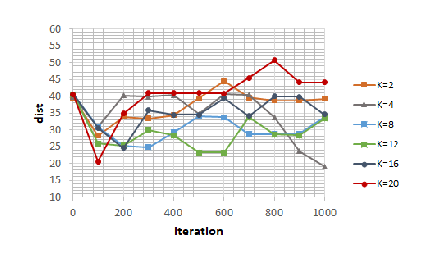
\includegraphics[width=0.4\textwidth]{eps/it-1_ns_r.eps}
\label{fig:rit_ns}}
\caption{Comparison with method II \& VI}
\label{fig:rit_iter}
\end{figure}

\begin{figure}[p]
\centering
\subfigure[k-NNBA]{
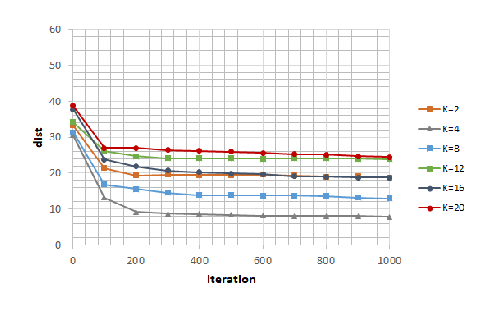
\includegraphics[width=0.4\textwidth]{eps/ip_k.eps}
\label{fig:i*_k}}

\subfigure[NSBA]{
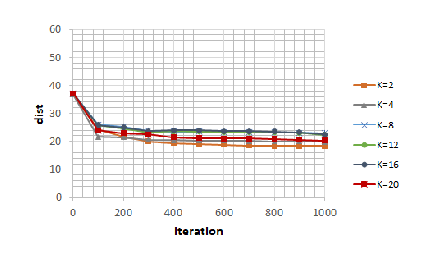
\includegraphics[width=0.4\textwidth]{eps/ip_ns.eps}
\label{fig:i*_ns}}
\caption{Comparison with method III \& VII}
\label{fig:i*_iter}
\end{figure}

\begin{figure}[p]
\centering
\subfigure[k-NNBA]{
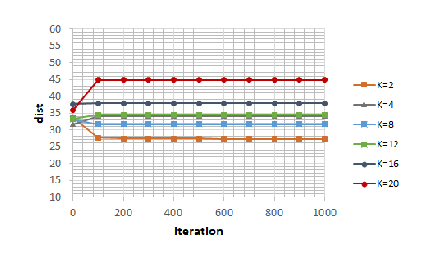
\includegraphics[width=0.4\textwidth]{eps/it-1_k.eps}
\label{fig:it_k}}

\subfigure[NSBA]{
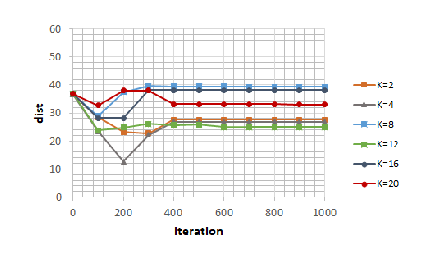
\includegraphics[width=0.4\textwidth]{eps/it-1_ns.eps}
\label{fig:it_ns}}
\caption{Comparison with method IV \& VIII}
\label{fig:it_iter}
\end{figure}

\begin{figure}[p]
\begin{center}
\begin{tabular}{c}
\begin{minipage}{0.5\hsize}
  \begin{center}
   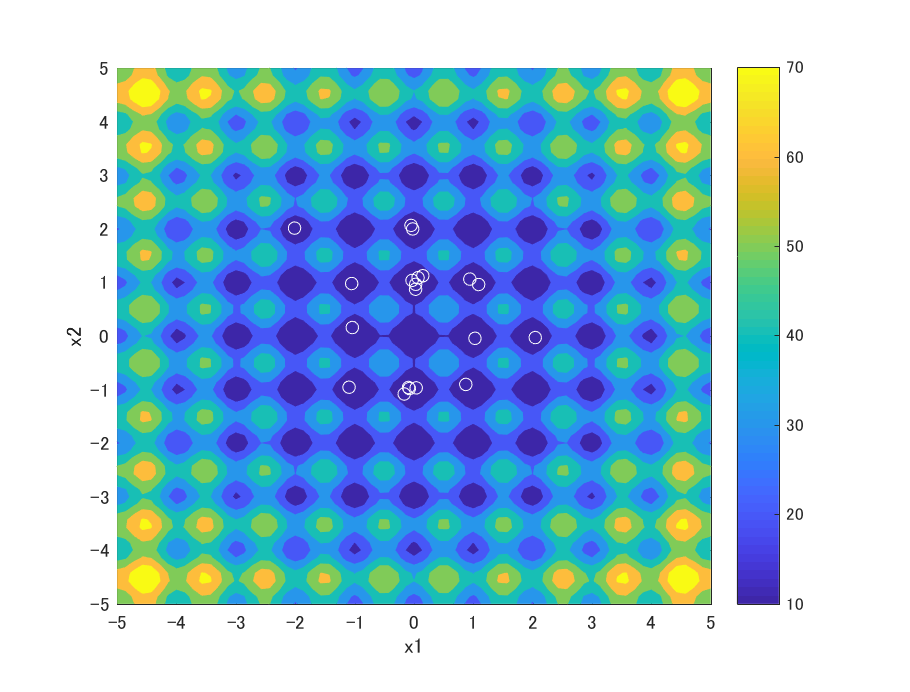
\includegraphics[width=45mm]{eps/i_k=4_1000.eps}
   \hspace{1.0cm} (a) k-NNBA
  \end{center}
  \label{fig:_k=4_i}
 \end{minipage}

 \begin{minipage}{0.5\hsize}
  \begin{center}
   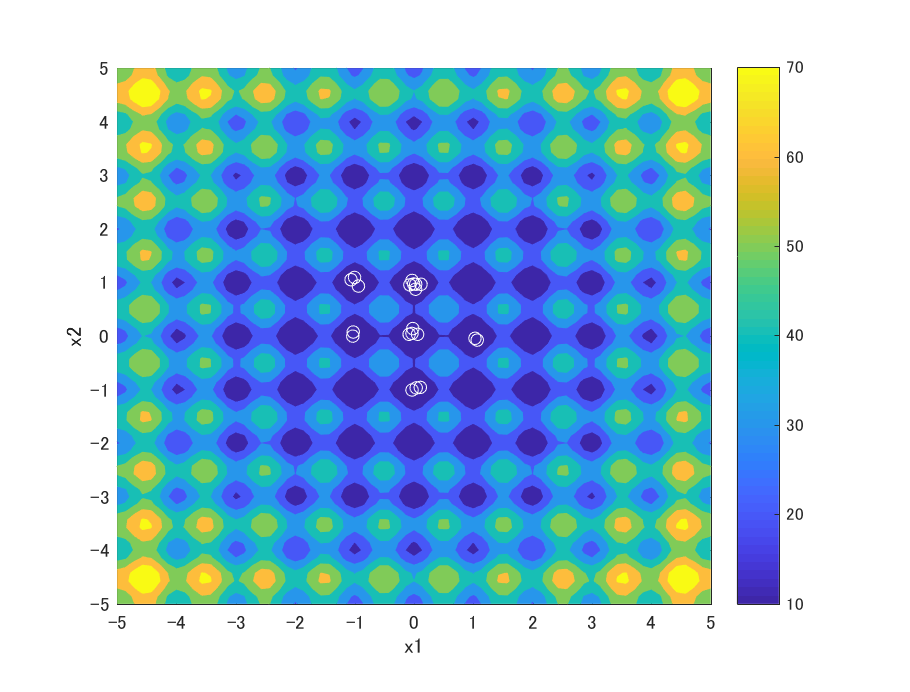
\includegraphics[width=45mm]{eps/v_k=4_1000.eps}
   \hspace{1.0cm} (b) NSBA
  \end{center}
  \label{fig:k=4_v}
 \end{minipage}
\end{tabular}
\end{center}
\caption{method I \& V (K=4)}
\label{fig:1000_15}
\end{figure}

\begin{figure}[p]
\begin{center}
\begin{tabular}{c}
\begin{minipage}{0.5\hsize}
  \begin{center}
   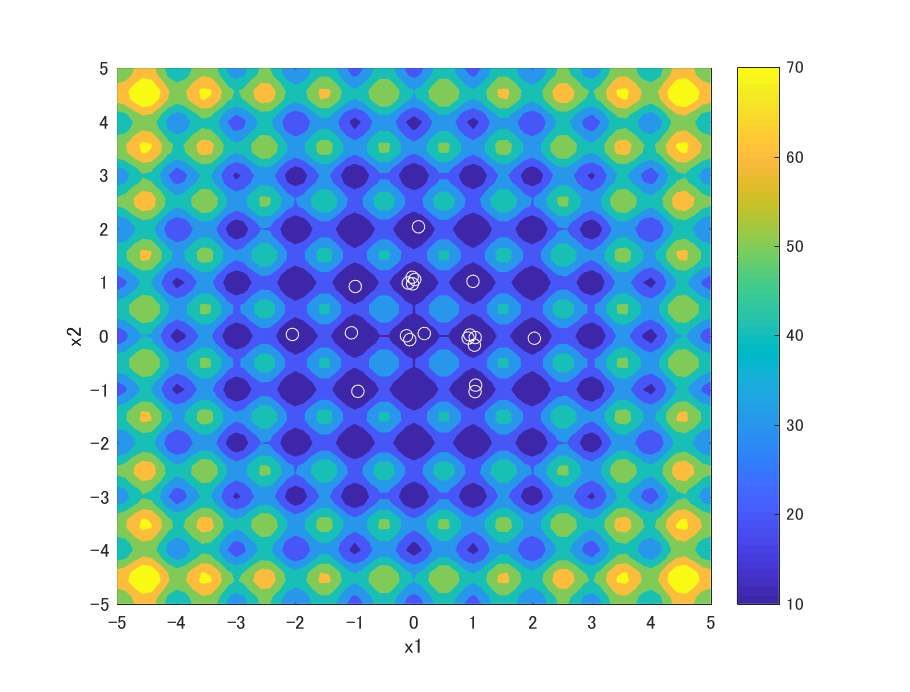
\includegraphics[width=45mm]{eps/ii_k=4_1000.eps}
   \hspace{1.0cm} (a) k-NNBA
  \end{center}
  \label{fig:k=4_ii}
 \end{minipage}

 \begin{minipage}{0.5\hsize}
  \begin{center}
   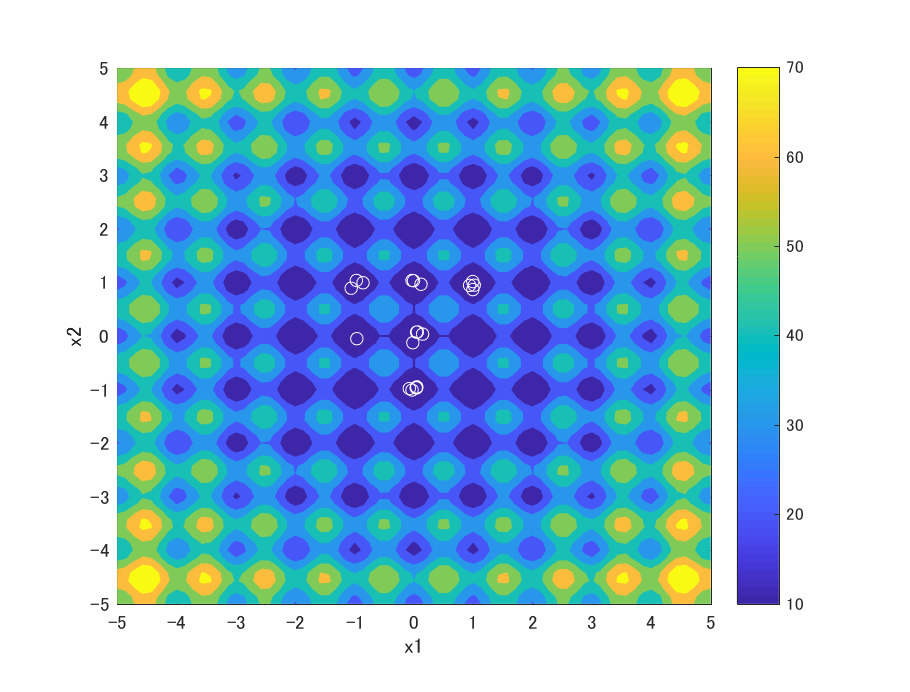
\includegraphics[width=45mm]{eps/vi_k=4_1000.eps}
   \hspace{1.0cm} (b) NSBA
  \end{center}
  \label{fig:k=4_vi}
 \end{minipage}
\end{tabular}
\end{center}
\caption{method II \& VI (K=4)}
\label{fig:1000_26}
\end{figure}

\begin{figure}[p]
  \begin{center}
\begin{tabular}{c}
\begin{minipage}{0.5\hsize}
  \begin{center}
   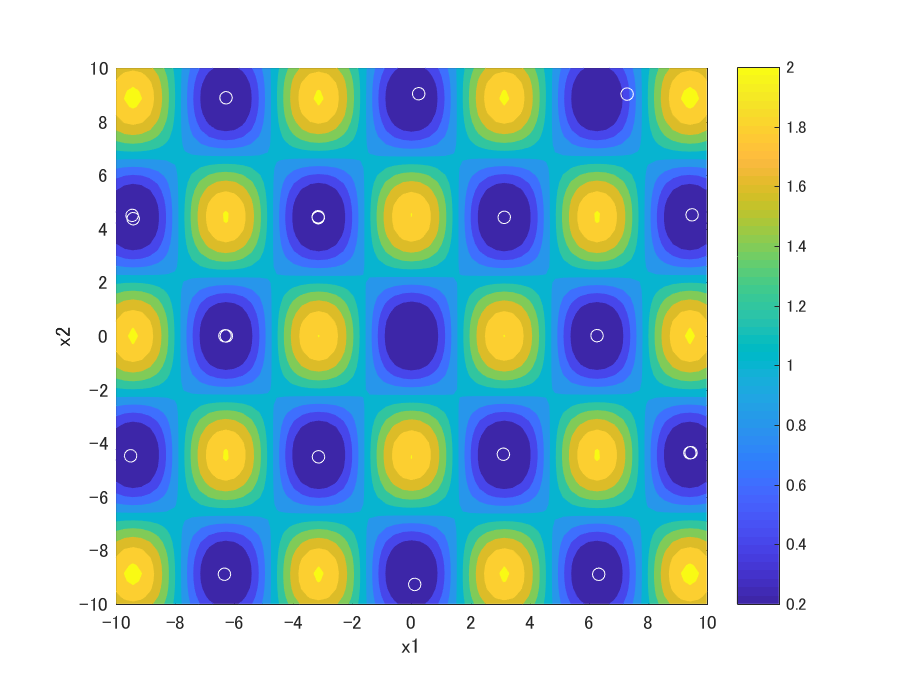
\includegraphics[width=45mm]{eps/iii_k=4_1000.eps}
   \hspace{1.0cm} (a) k-NNBA
  \end{center}
  \label{fig:k=4_iii}
 \end{minipage}

 \begin{minipage}{0.5\hsize}
  \begin{center}
   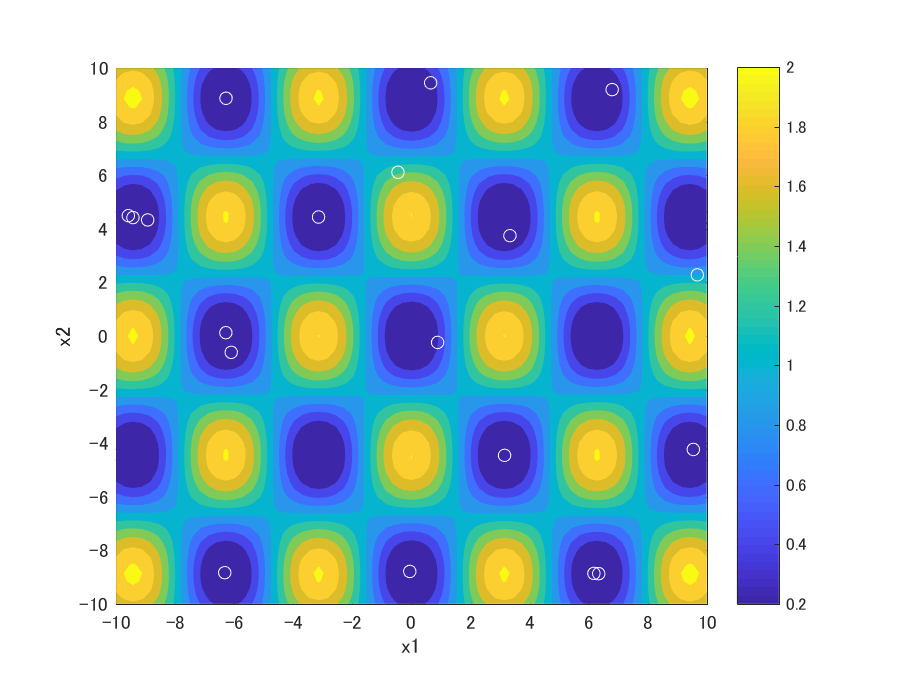
\includegraphics[width=45mm]{eps/vii_k=4_1000.eps}
   \hspace{1.0cm} (b) NSBA
  \end{center}
  \label{fig:k=4_vii}
 \end{minipage}

\end{tabular}
\caption{method III \& VII (K=4)}
\label{fig:1000_37}
\end{center}
\end{figure}

\begin{figure}[p]
\begin{center}
\begin{tabular}{c}
\begin{minipage}{0.5\hsize}
  \begin{center}
   \includegraphics[width=45mm]{eps/iv_k=4_1000.eps}
   \hspace{1.0cm} (a) k-NNBA
  \end{center}
  \label{fig:k=4_iv}
 \end{minipage}

 \begin{minipage}{0.5\hsize}
  \begin{center}
   \includegraphics[width=45mm]{eps/viii_k=4_1000.eps}
   \hspace{1.0cm} (b) NSBA
  \end{center}
  \label{fig:k=4_viii}
 \end{minipage}
\end{tabular}
\end{center}
\caption{method IV \& VIII (K=4)}
\label{fig:1000_48}
\end{figure}


\section{Discussion}
There are line graphs for all methods on Griewank function. The horizontal axis describes iteration of evaluating solutions, and vertical axis describes the sum of distance between each local minima and the closest solution shown as Fig. \ref{fig:ri*_iter} to \ref{fig:it_iter}. Besides distributed solutions at 1000th iteration from Fig. \ref{fig:1000_15} and \ref{fig:1000_26} for rastrigin function from Fig. \ref{fig:1000_37} and \ref{fig:1000_48} for griewank function. 
\subsection{k-NNBA vs NSBA}
From Fig. \ref{fig:rtbar_func} to \ref{fig:tbar_func}, k-NNBA tends to decline as neighbors increase. NSBA is hardly affected by changes of neighbors, so that it performed better than k-NNBA relatively. Especially in k=4 from Fig. \ref{fig:1000_15}, \ref{fig:1000_26} and \ref{fig:1000_48}, k-NNBA more distributed than NSBA obviously. It means that equation of considering distance still performed weakly. For this reason, we have to adjust the number of neighbors and population size and updating equation.
  
\subsection{Existence or nonexistence of ${x_{rnd}}$}
Compared line graph with Fig. \ref{fig:ri*_iter} \& \ref{fig:rit_iter} and Fig. \ref{fig:i*_iter} \& \ref{fig:it_iter}, ${x_{rnd}}$ affected iteration. Especially in Fig. \ref{fig:ri*_iter} \& \ref{fig:it_iter}, ${dist}$ fluctuated until 1000 iterations in any neighbors. By contrast in Fig. \ref{fig:i*_iter} \& \ref{fig:it_iter}, ${dist}$ of any neighbors became stable over a certain iteration. 

\subsection{Differences in ${x_i^{t-1}}$ and ${x_{i*}}$}
Focused on 4 line graphs in right side Fig. \ref{fig:i*_iter} and \ref{fig:it_iter} without ${s_{rnd}}$, ${x_{i*}}$ indicates personal best solution, these ${dist}$ fell continuously until 300 iterations and became stable to the end. From left side in Fig. \ref{fig:ri*_iter} \& \ref{fig:rit_iter}, all ${dist}$ fluctuated constantly, as ${x_{rnd}}$ has strong effect on iteration.

\section{Conclusion}
We validated the performance of proposed bat algorithms for k-nearest neighbor and novelty search with changes of updating solutions and generating a new solution randomly. As a result, both algorithms performed for reaching local minima with global optimum. Especially the method using personal best without ${s_{rnd}}$, performed better than the other proposed methods. However, we have to adjust parameter k which is the number of neighbors for feasible multimodal functions. As population size of bat increases, the number of searched local minima  also increased. Our future prospects are adapting this algorithm for the other benchmark functions, and blushing up the performance to cover unspecified large number of local minima. Future experiments on the other multimodal functions and investigation will be studied.

\begin{thebibliography}{99}
\bibitem{PSO01}
Eberhart, R. C., and Kennedy: A New Optimizer Using Particle Swarm Theory,
\textit{Proc. Sixth International Symposium on Micro Machine and Human Science (Nagoya, Japan), IEEE Service center, Pis-cataway, NJ}, No.~1, pp.~39--43, 1995.
\bibitem{FA01}
Yang, X. S: Firefly Algorithms for Multimodal Optimization,
\textit{in:Stochastic Algorithms: Foundations and Applications, SAGA}, Vol.~5792, pp.~169--178, 2009.

\bibitem{BA01}
Yang, X. S.: A Metaheuristic Bat-Inspired Algorithm,
 \textit{in: Nature Inspired Cooperative Strategies for Optimization(NICSO 2010), Springer, Berlin}, Vol.~284, pp.~65--74, 2010.

% \bibitem{PSO4mo}
% J. H. Seo, C. H. Lim, C. G. Heo, J. K. Kim, H. K. Jung and C. C. Lee: Multimodal Function Optimization Based on Particle Swarm Optimization, \textit{IEEE Transactions on Magnetics},  Vol.42, pp.1095-1098, No.4, 2006.

% \bibitem{PSO4mo2}
% B. Y. Qu, P. Suganthan, and S. Das: A Distance-Based Locally Informed Particle Swarm Model for Multimodal Optimization, \textit{IEEE Transactions on Evolutionary Computation}, Vol.17, pp. 387-402, No.3, 2013.

% \bibitem{DE4mo}
% Thomsen, R.: Multimodal  Optimization using crowding-based differential evolution,
% \textit{IEEE Congress on Evolutionary Computation}, Vol.2, pp.1382--1389, 2004.

% \bibitem{DE4mo2}
% Li, X. : Efficient differential evolution using speciation for multimodal function optimization, \textit{GECCO Proceedings of the 7th annual conference on Genetic and evolutionary computation}, pp.873-880, 2005.

% \bibitem{GPharada}
% S. Yoshida, T. Harada, and R. Thawonmas: Multimodal Genetic Programming by Using Tree Structure Similarity Clustering, \textit{IEEE 10th International Workshop on Computational Intelligence and Applications, (Hiroshima, Japan)}, 2017.
\end{thebibliography}

\end{document}
